% replace all text with your own text.
% in this template few examples are mention
\chapter{Methodology}
\label{ch:method} % Label for method chapter


\section{Working with the Tweets Dataset}

\subsection{Explorartory Data Analysis}

\textbf{Number of Words in Tweets:}
To understand the distribution of the number of words in tweets, we plotted histograms for disaster and not-disaster tweets. The histogram for tweets shows a peak around 15-20 words. Also histogram indicates that not disaster-related tweets may be slightly longer scentences on average compared to non-disaster tweets.

\begin{figure}[ht]
    \centering
    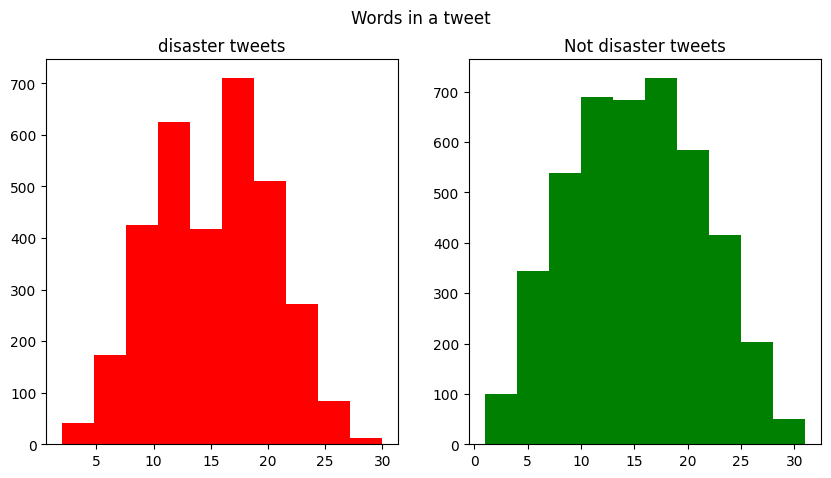
\includegraphics[scale=0.7]{figures/numberofwords.png}
    \caption{Number of words in the tweets based on class}
\end{figure}

\newpage
\textbf{Punctuations in Tweets:}
We analyzed the usage of punctuations in tweets, separating disaster and non-disaster tweets. The histograms displayed the frequency of various punctuation marks such as commas, exclamation marks, and hashtags. Disaster tweets tend to have more question marks and hashtags compared to non-disaster tweets, suggesting a more urgent or expressive tone.

\begin{figure}[ht]
    \centering
    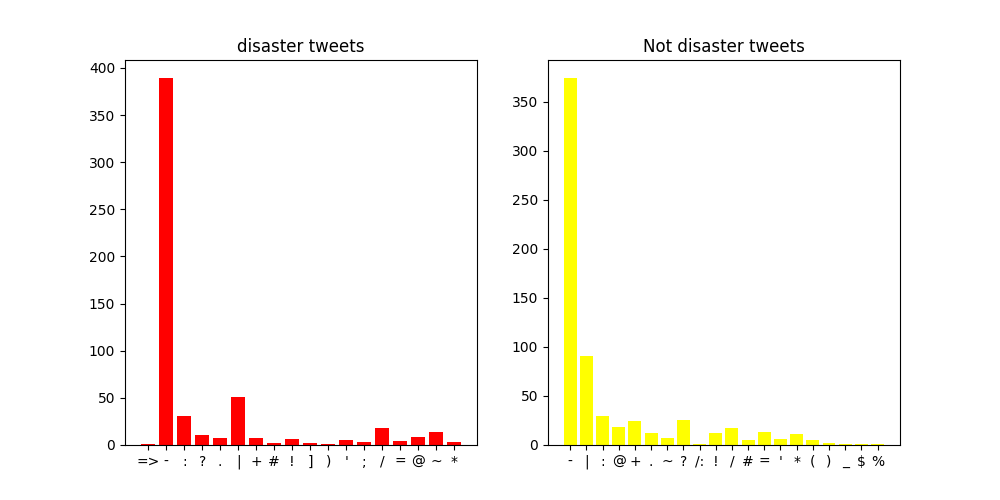
\includegraphics[scale=0.7]{figures/punctuationfor1.png}
    \caption{Punctuations in the tweets based on class}
\end{figure}

\textbf{Bigrams Analysis:}
Bigrams analysis revealed common pairs of words occurring together in tweets. The bigrams showed the preposition of the places like "in the", "on the".
"to be",indicating discussions about readiness and safety measures.
"for the" bigram suggesting discussions about response efforts and support for affected individuals. This analysis provides insights into the topics and contexts discussed in disaster-related content.

Notably, the bigram "http co" appeared frequently, indicating the presence of URLs and links that require cleaning and removal from the tweet text. Handling these URLs is crucial as they often do not contribute to the analysis of tweet content and can introduce noise.
\begin{figure}[ht]
    \centering
    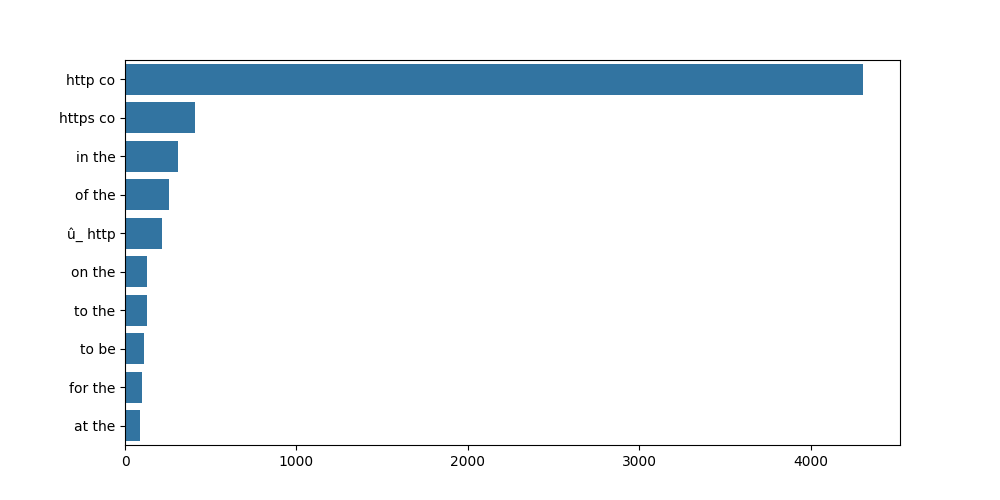
\includegraphics[scale=0.7]{figures/bigram.png}
    \caption{Bigrams in the tweet}
\end{figure}

\newpage
\textbf{Common Words in Tweets:}
By identifying the most common words, you can gain insights into the overall themes and topics present in the tweets. This helps in understanding the nature of the data and what it predominantly talks about. In some cases, analyzing common words can also help in quality assurance by identifying anomalies, spammy content, or irrelevant data that might need further investigation or filtering.
\begin{figure}[h]
    \centering
    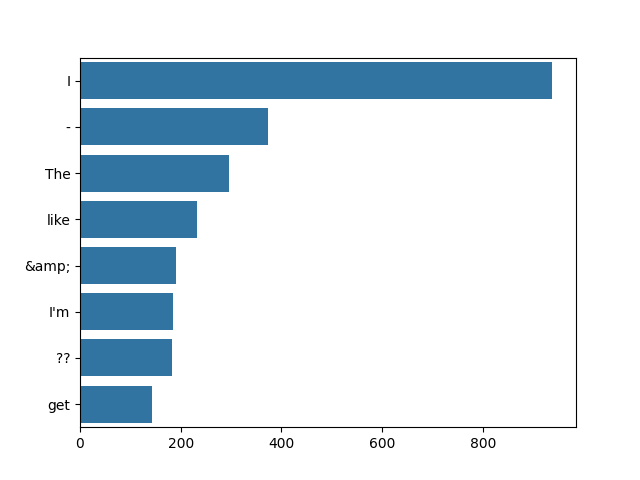
\includegraphics[width=0.5\textwidth]{figures/commonwords.png}
    \caption{Common words in the tweets}
\end{figure}


\clearpage
\subsection{Data Cleaning}

\textbf{Removing URLs}
We started by removing URLs from the tweet text as they often don't contribute to the analysis of tweet content and can introduce noise.

\textbf{Removing Punctuations}
Next, we removed punctuations such as commas, periods, and exclamation marks from the text. This step helps in standardizing the text data and focusing on the actual words and meanings in the tweets.
\begin{figure}[ht]
    \centering
    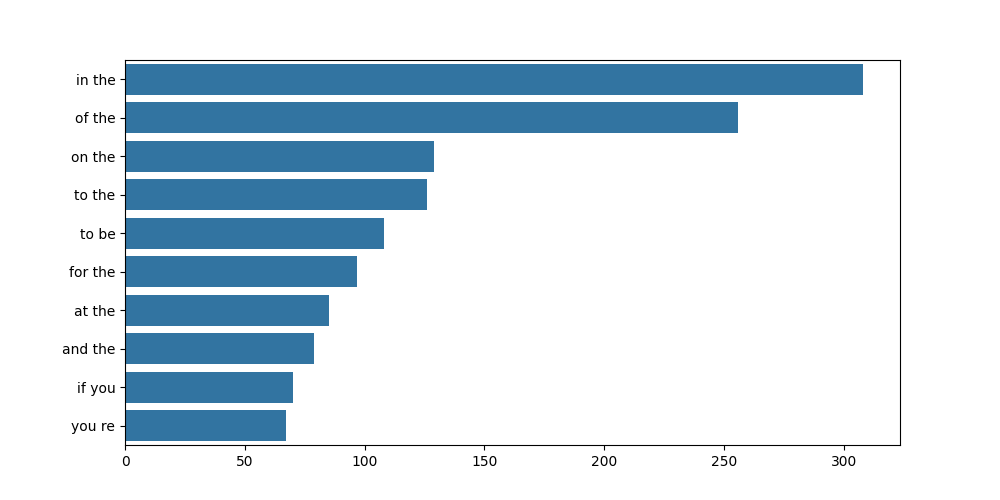
\includegraphics[scale=0.7]{figures/CleanedDatabigram.png}
    \caption{Bigram after datacleaning}
\end{figure}

\newpage
\textbf{Word Cloud after Data Cleaning}
After data cleaning, we generated a word cloud to visualize the most common words in disaster-related tweets. This visualization helps in understanding the key themes and topics prevalent in the cleaned tweet data. Using a word cloud and bar plot, we identified the most common words in disaster-related tweets. Terms like "fire," "disaster, "shelter" appeared prominently, reflecting the focus on urgent situations and crises in these tweets.

These exploratory data analysis and data cleaning steps are crucial for preprocessing the tweet data and gaining insights into the characteristics of disaster-related content on social media platforms.
\begin{figure}[ht]
    \centering
    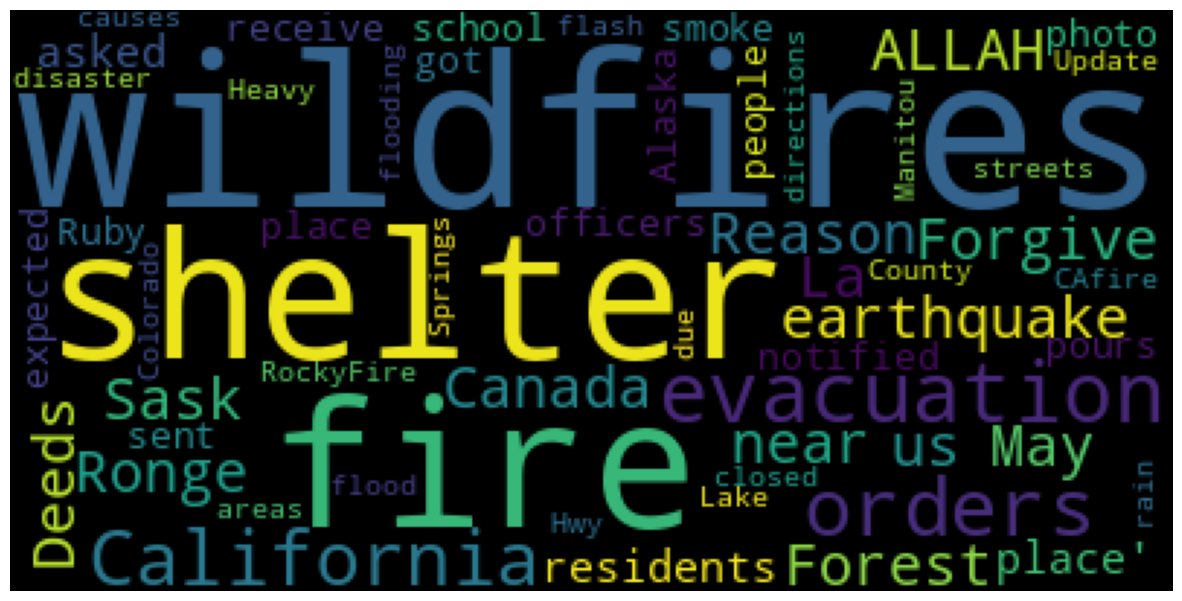
\includegraphics[scale=0.5]{figures/wordcloud.png}
    \caption{Wordcloud for tweets data}
\end{figure}

\newpage
\section{Algorithms}


\subsection{Logistic regression for tweet classification}
Logistic regression is a linear classification algorithm used extensively for binary classification tasks, where the goal is to predict a binary outcome (e.g., disaster or non-disaster) based on input features (e.g., tweet text).

\textbf{Text Preprocessing and Vectorization:}
Text Tokenization:The tweet text is tokenized, breaking it down into individual words or tokens. Count Vectorization: The CountVectorizer is used to convert the tokenized text into numerical vectors. Each tweet is represented by a vector where each element corresponds to the count of a specific word in the tweet.

\textbf{Dataset Splitting:}
The dataset is split into training and validation sets using a predefined ratio (e.g., 80 percent for training, 20 percent validation).
This separation allows us to train the model on a subset of data and evaluate its performance on unseen data.

\textbf{Training Process:}
The model is trained using the training data and their corresponding vector representations. During training, the model adjusts its coefficients to minimize the logistic loss function and improve classification accuracy.

\textbf{Performance Evaluation:}
The model's accuracy on the training set is calculated to assess its performance on data it has been trained on. Training accuracy indicates how well the model fits the training data. The model's accuracy on the validation set is computed to evaluate its generalization ability to unseen data.
Validation accuracy helps determine if the model can make accurate predictions on new tweets.

\newpage
\textbf{Confusion Matrix Analysis:}

The confusion matrix is generated to visualize the model's predictions on both the training and validation sets.
It consists of four quadrants: true positives (TP), true negatives (TN), false positives (FP), and false negatives (FN).

\textbf{F1 Score Calculation:}

The F1 score, which combines precision and recall, is calculated based on the confusion matrix.
It provides a single metric to assess the model's overall performance, particularly useful for imbalanced datasets.


\begin{figure}[ht]
    \centering
    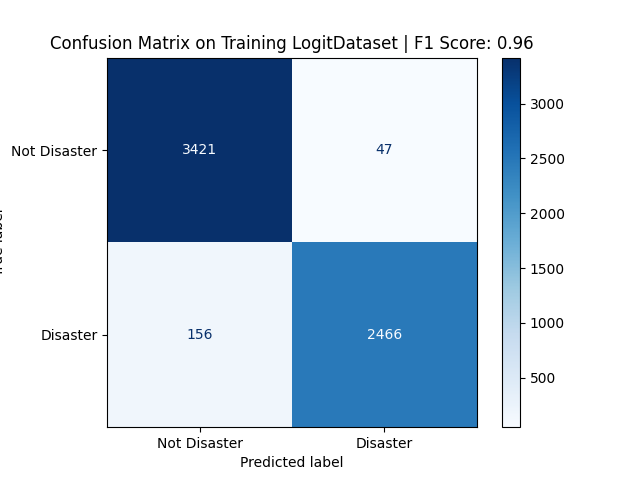
\includegraphics[scale=0.7]{figures/LogisticRegression_Training Logit_confusion_matrix.png}
    \caption{Wordcloud for tweets data}
\end{figure}

\begin{figure}[ht]
    \centering
    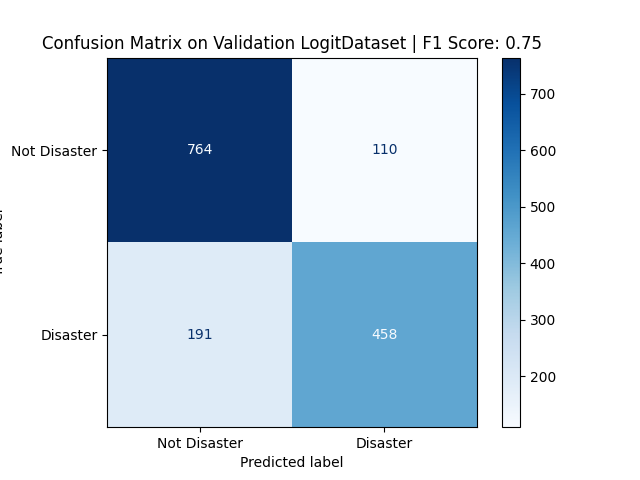
\includegraphics[scale=0.7]{figures/LogisticRegression_Validation Logit_confusion_matrix.png}
    \caption{Wordcloud for tweets data}
\end{figure}

\newpage
\subsection{DistilBERT for tweet classification}

DistilBERT is a state-of-the-art transformer-based model designed for natural language processing (NLP) tasks, particularly well-suited for tweet classification, such as identifying disaster-related tweets from non-disaster ones.

\textbf{DistilBERT Model Configuration}
Preprocessing:
The DistilBERT model uses a preprocessor specifically tailored for tweet analysis, with a preset configuration for handling tweet sequences up to 160 tokens in length.


\textbf{Model Architecture:}

The DistilBERT classifier is based on the "distil bert base en uncased" preset, which utilizes a distilled version of the BERT (Bidirectional Encoder Representations from Transformers) architecture. This architecture incorporates transformer layers to process input tokens, capturing contextual relationships between words and phrases in the tweet.
The "distilbert-base-uncased" denotes a base-sized variant of the DistilBERT model that was trained using uncased text data. This model finds widespread application across a range of natural language processing tasks like text classification, sentiment analysis, question answering, among others.

\textbf{Training the model:}
The training setup includes a batch size of 20, a training split of 80, and a validation split of 20 to ensure robust model evaluation.
The number of training examples is determined dynamically from the dataset, and the number of steps per epoch is calculated based on the batch size and training examples. To maintain reproducibility, a random seed of 0 is set before training the model, ensuring consistent results across different runs.

\textbf{Model Summary}

The DistilBERT model summary provides insights into the model architecture, including the number of layers, parameters, and output shapes.
This summary aids in understanding the complexity and capabilities of the DistilBERT classifier for tweet analysis.
The classifier is trained over 7 epochs, optimizing the model using the Adam optimizer with a learning rate of 1e-5.
During training, performance metrics such as accuracy and loss are monitored to assess the model's learning progress.
Evaluation includes validating the model's performance on a separate validation set to gauge its ability to generalize to unseen data.

\begin{figure}[ht]
    \centering
    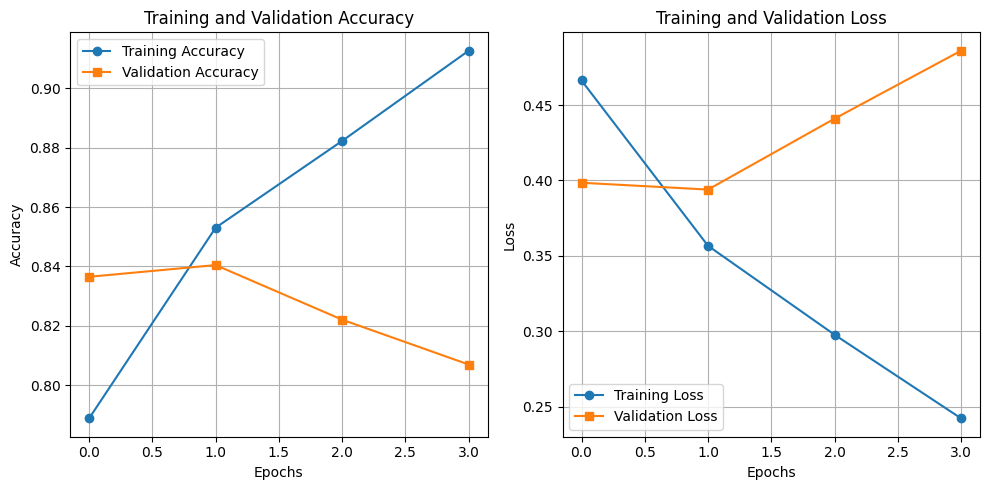
\includegraphics[scale=0.7]{figures/noautotune_trainingValidation.png}
    \caption{Distilbert with parameter setting accuracy and loss graph}
\end{figure}

\begin{figure}[ht]
    \centering
    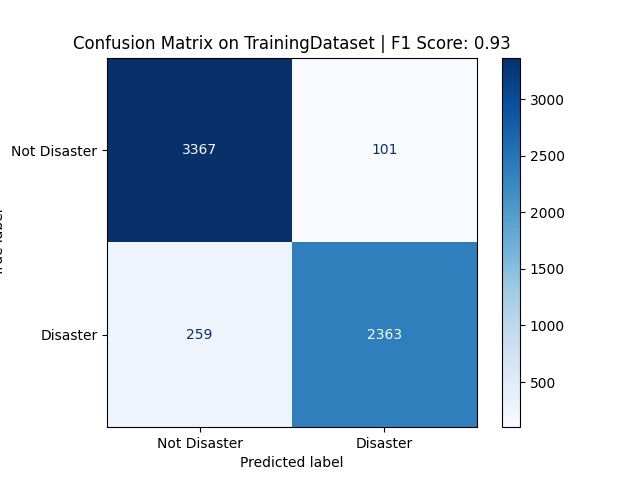
\includegraphics[scale=0.7]{figures/Distilbert_Training_confusion_matrix.png}
    \caption{Distilbert with parameter setting}
\end{figure}

\begin{figure}[ht]
    \centering
    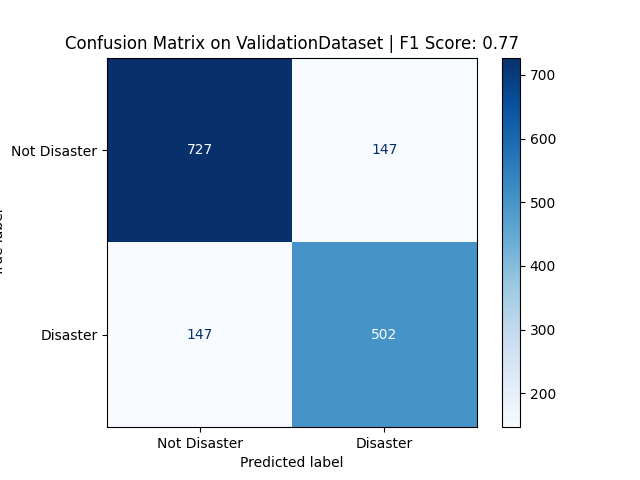
\includegraphics[scale=0.7]{figures/Distilbert_Validation_confusion_matrix.png}
    \caption{Distilbert with parameter setting}
\end{figure}

\newpage
\textbf{DistilBert with Autotune}

Efficient data loading and processing are critical aspects of training deep learning models, especially when working with large datasets. TensorFlow, a popular deep learning framework, provides the AUTOTUNE feature to dynamically optimize data loading and preprocessing operations, enhancing training performance and resource utilization.

\textbf{The Need for Optimization:}

In deep learning workflows, data loading and preprocessing pipelines can become bottlenecks, slowing down model training and inference. These pipelines involve tasks such as reading data from storage, applying transformations (e.g., augmentation, normalization), and preparing batches for training. Traditional approaches often involve static configurations for these operations, which may not fully exploit system resources or adapt to varying workloads.

\textbf{Understanding AUTOTUNE:}

TensorFlow's AUTOTUNE feature addresses these challenges by enabling dynamic optimization of data loading and processing. When applied to dataset operations, AUTOTUNE allows TensorFlow to automatically adjust parameters such as parallelism, prefetching, and buffer sizes based on system conditions and available resources.

By setting prefetch(tf.data.AUTOTUNE) on these datasets, TensorFlow dynamically optimizes data loading and preprocessing operations during model training.

\textbf{Benefits of AUTOTUNE:}

Optimized Parallelism: AUTOTUNE adjusts parallelism settings to exploit multi-core CPUs or GPUs efficiently, reducing data loading bottlenecks and improving training throughput.
Dynamic Prefetching: TensorFlow prefetches batches of data ahead of time, overlapping data loading with model computation. AUTOTUNE optimizes the prefetch buffer size based on system performance, reducing training latency.
Resource Utilization: By adaptively tuning parameters such as buffer sizes and parallelism, AUTOTUNE optimizes resource utilization, preventing underutilization or resource contention during training.
Conclusion:

The use of AUTOTUNE in TensorFlow significantly enhances the efficiency of data loading and preprocessing pipelines in deep learning workflows. By dynamically optimizing parameters based on system conditions, AUTOTUNE improves training performance, accelerates convergence, and maximizes resource utilization, making it a valuable tool for deep learning practitioners.

\begin{figure}[ht]
    \centering
    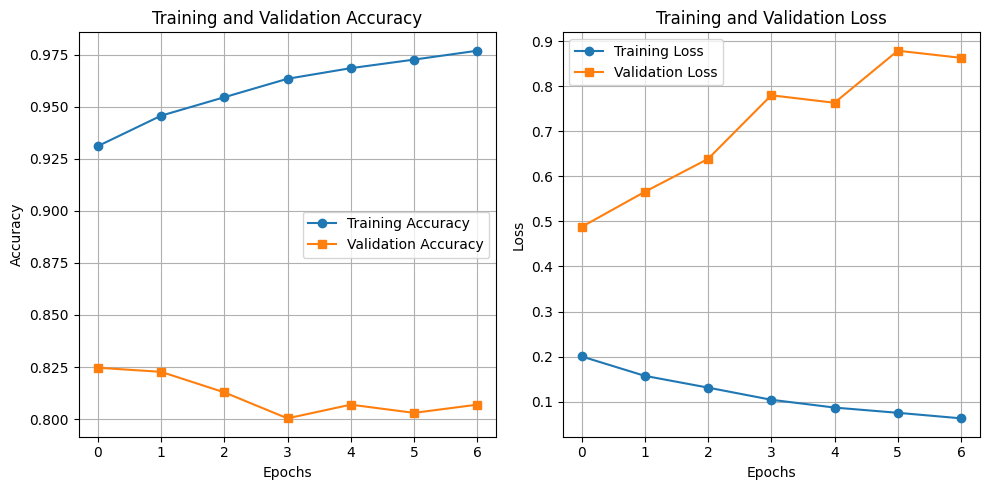
\includegraphics[scale=0.7]{figures/autotune_trainingValidation.png}
    \caption{Distilbert with autotune accuracy and loss graph}
\end{figure}

\begin{figure}[ht]
    \centering
    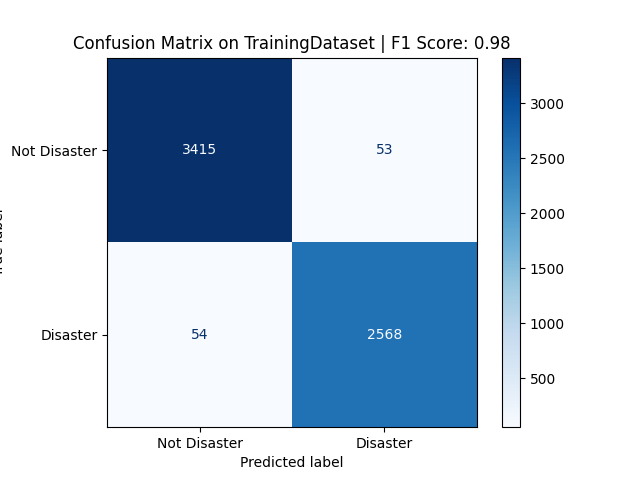
\includegraphics[scale=0.7]{figures/Distilbert_autotune_Training_confusion_matrix.png}
    \caption{Distilbert with autotune}
\end{figure}

\begin{figure}[ht]
    \centering
    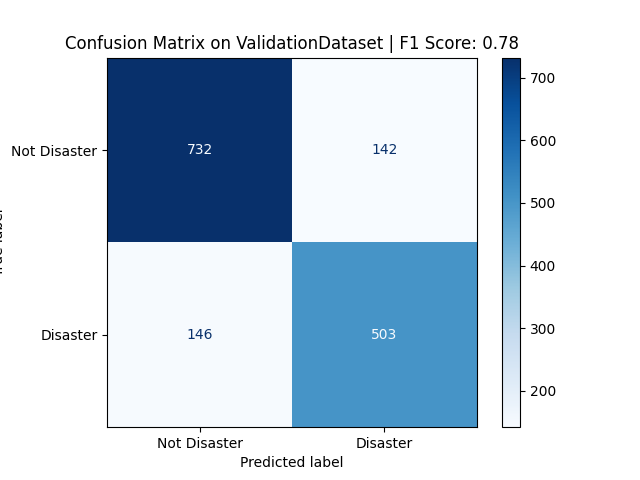
\includegraphics[scale=0.7]{figures/Distilbert_autotune_Validation_confusion_matrix.png}
    \caption{Distilbert with autotune}
\end{figure}

\newpage
\section{Summary}
Logistic regression is suitable for simpler text classification tasks, offering interpretability and efficiency, whereas DistilBERT excels in capturing complex patterns and semantics, albeit at the cost of increased computational resources and complexity. The choice between the two depends on the task complexity, dataset size, interpretability requirements, and available computational resources.

The DistilBERT model benefits from this optimization, ensuring that computational resources are utilized effectively during training and inference.
Overall, the configuration and training setup of the DistilBERT model for tweet analysis demonstrate a methodical and optimized approach, leveraging state-of-the-art NLP techniques to achieve accurate classification of disaster-related tweets.



